
\documentclass[a4paper]{article}

\usepackage[english]{babel}
\usepackage[utf8]{inputenc}
\usepackage{csquotes}
\usepackage{amsmath}
\usepackage{graphicx}
\usepackage{hyperref}

% Load in biblatex
% To use a different bibliography style, just change "numeric" to
% your preferred style (mla for MLA style, alphabetic for Author-Year
% style, etc.) There are a lot of options; check the BibLaTeX documentation.
\usepackage[backend=bibtex8,style=numeric]{biblatex}
%% Select the bibliography file
%\addbibresource{sources.bib}


\title{Diploma Thesis\\Tasks Results}
\author{Andreas Egger \\0626885}
\date{Technical University of Vienna}


\begin{document}
\maketitle

\newpage

\tableofcontents

\newpage

\section{Outlining simulation}
\hfill\date{Week 07.04. to 13.04.}

\subsection{Defining simulation conditions}

\begin{itemize}

\item Defining countries and locations of data centers

There will be seven data centers located in seven different countries, each belonging to a specific energy market. 

Below is an outline of countries and cities of data center locations grouped by the corresponding energy markets. 

	\subitem European Energy Exchange (EEX) 
	
		\subsubitem - Germany: Berlin
		
		\subsubitem - Switzerland: Zurich
		
		\subsubitem - France: Paris
		
	\subitem Nord Pool Spot Market 
	
		\subsubitem - Finland: Helsinki
		
	\subitem APX Power Spot Market
	
		\subsubitem - England: London
		
	\subitem ISO New England
	
		\subsubitem - Maine: Portland
		
		\subsubitem - Massachusetts: Boston

\item Creating a visual outline of the geographical structure

A basic outline of the simulation scenario is shown in Figure~\ref{fig:simulation-outline}. 

The figure depicts a private cloud of a mid-sized company comprising several data centers distributed across different countries. 
%Basically there are seven data centers distributed across several countries. 
The dashed lined boxes group the data centers to the respective power market they belong to. The data centers are interconnected in a way that data may be transferred between any two data centers. 

Since data centers are distributed across Europe and the east coast of North America, interesting constellations may arise in terms of time and location based energy pricing and temperature levels, which may influence the amount of cooling needed which in turn affects the amount of power consumption needed for a specific data center, respectively. 


\begin{figure}[htbp]
	\centering
		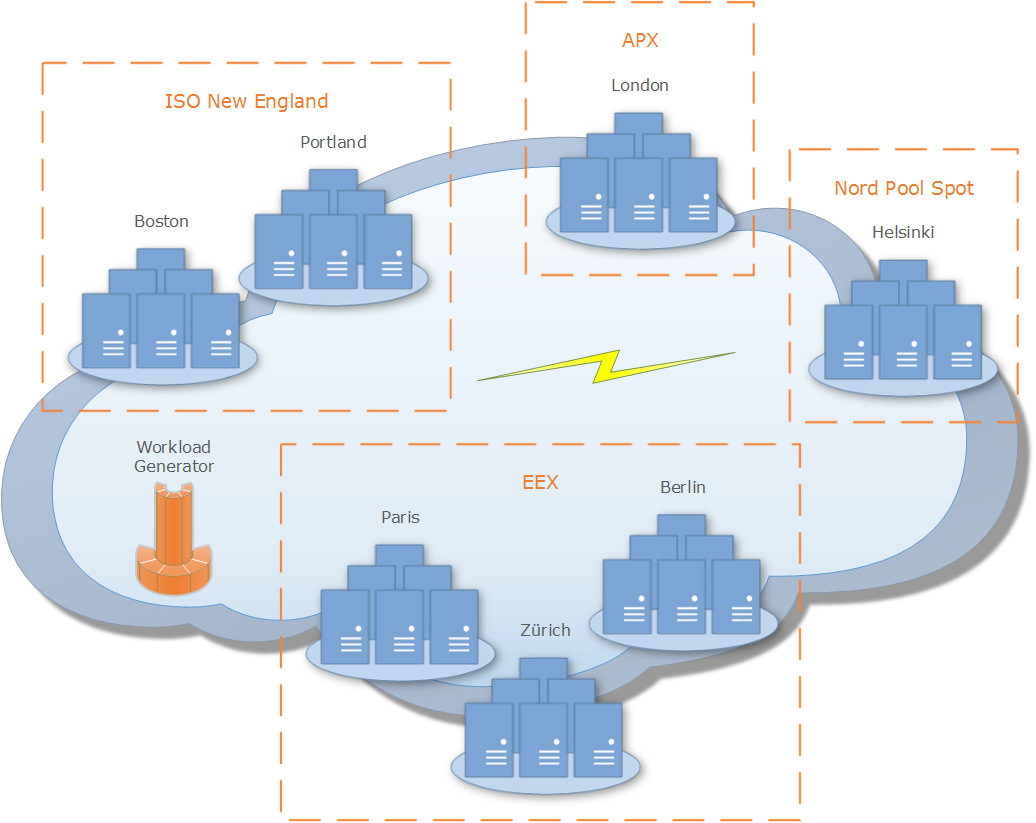
\includegraphics[width=1.00\textwidth]{images/simulation_outline.png}
	\caption{Visual outline of the simulation scenario}
	\label{fig:simulation-outline}
\end{figure}




\item Defining parameters of the simulation

\emph{To be defined:}

	\subitem Data Center
	
		\subsubitem - Number of servers
		
		\subsubitem - Type of servers (CPU power, power draw)
		
		\subsubitem - Size of data center
		
		\subsubitem - Total power costs
	
	\subitem Cooling infrastructure
	
		\subsubitem - Number of Fans and/or Chillers per data center
		
		\subsubitem - Speed, trigger points related to outside temperature
		
		\subsubitem - Consider startup time
	
	\subitem Type of workload
		
		\subsubitem - Long running, data intensive workload
		
		\subsubitem - Short running requests
		
		\subsubitem - Simulating CPU usage behaviour
		
	\subitem Workload Generator (Load Balancer)
			
		\subsubitem - Responsible for distributing request to data centers
		
		\subsubitem - Decides on type of request
		
		\subsubitem - Current / future conditions (energy price, temperature levels) 
		
	\subitem Forecasting
	
		\subsubitem - short term (one day to a few days ahead)
		
		\subsubitem - specify methods in detail
		
	\subitem SLAs
	
		\subsubitem - allowable delay of tasks in seconds
		
		\subsubitem - minimum CPU power overhead for tasks in cycles

	\subitem Migration / Overhead costs
	
		\subsubitem - migrating VMs between data centers
		
		\subsubitem - Cost depending on distance, amount of data
		
	\subitem Minimum number of VMs to migrate
	
		\subsubitem - depending on migration costs and energy prices
			
	\subitem Power consumption behavior
	
		\subsubitem - Idle Servers
		
		\subsubitem - Partially utilized Servers (max. 1, negligible)
		
		\subsubitem - Fully utilized Servers
	
	\subitem Different kinds of energy sources
	
		\subsubitem - Renewables, Atom, Fossils
		
		\subsubitem - Possibly prioritizing green IT over price

	\subitem Definition On/Off Peak Prices
	
		\subsubitem - depending on respective power market
		
		\subsubitem - considering relevant time zones
		
	\subitem Different Timezones (By countries)

		\subsubitem - Maine, Massachusetts (-5) 

		\subsubitem - UK (UTC) 

		\subsubitem - Germany, France, Switzerland (+1) 

		\subsubitem - Finland(+2)
		
	
		

\item Collecting energy price data from the various energy markets

	\subitem European Energy Exchange
	
	EEX sets the energy prices for the countries in middle Europe and is an important platform for electricity price trading.  
	Data is available for the areas Switzerland, Germany/Austria and France, each describing a different part of the power market. It can be ordered and downloaded from an ftp server.
	
	website: \url{http://www.eex.com/}
	
	\subitem Nord Pool Spot Market
	
	The Nord Pool Spot Market is the largest power spot market in the world, with participating countries Norway, Denmark, Sweden, Finland, Estonia, Latvia and Lithuania. It contains three spot markets, Elspot, Elbas and N2EX  whereby Elspot is the most common one. It features different energy data attributes like Flow, Prices, Volumes and Capacities. It has a wide variaty of data available for the different countries. 
	
	website: \url{http://www.nordpoolspot.com/}
	
	\subitem APX Power Spot Exchange
	
The APX Power Spot market provides energy price data from the UK and the Netherlands. It comprises daily results and historical market data. Prices are given in Pounds. 

	website: \url{http://www.apxgroup.com/}

	\subitem ISO New England
	
	ISO New England contains data comprising the countries of the New England association, namely Connecticut, New Hampshire, Maine, Massachusetts, Rhode Island und Vermont. Two countries have been selected, Massachusetts and Maine, for which data is readily available. 
	
	website: \url{http://www.iso-ne.com/}

\item Examining data formats and ways to process them

	\subitem European Energy Exchange
	
	EEX offers infoproduct packages to get historical intraday spot prices and power future contracts (derivatives) for the years 2000 and 2002 until today, depending on the offered data format. 
	It provides its data in csv, xml and xls, partly containing different information. It is separated by year and country or market area, respectively. 
	

	\subitem Nord Pool Spot Market
	
	For the Nord Pool Spot Power market there are a number of data sets publicly available, however only from 2012 onwards. 
	The markets offer information about flow, price, volume and capacities in the given year. The Elspot market provides hourly, daily and weekly data, again freely available from 2012 onwards in files containing different nordic currencies.  

	\subitem APX Power Spot Exchange
	
	At APX Power Exchange just like at EEX data is provided via an ftp server. In order to get access one has to subscribe by email, responses are now on their way. 
	
	\subitem ISO New England
	
	At the ISO New England Power Spot market one can choose different types of historical energy price data, namely five-minute data, hourly data, daily data and monthly data. In addition there is data about short and long term outages available. 
	Data is given both in csv and xls format, for easy processing. 

\end{itemize}



\vspace{1em}

\hfill\date{Week 16, from 14.04. to 20.04.}

\section{Forecasting}

\subsection{Experiment on forecasting methods}

\begin{itemize}

\item Examine the forecasting methods in relation to the actual energy price data

\item Finding metrics for accuracy of the methods

\item Setting up a test environment for testing forecasts

\item Test forecasting for different time ranges (day ahead, few days)

\item Compare the accuracy of forecasts for different models

\end{itemize}


\end{document}